\documentclass[tikz,border=5pt]{standalone}
\usepackage{pgfplots}
\pgfplotsset{compat=1.18}

\definecolor{corba}{HTML}{365FB3}
\definecolor{punt}{HTML}{B91C1C}
\definecolor{guia}{HTML}{6B7280}

\begin{document}
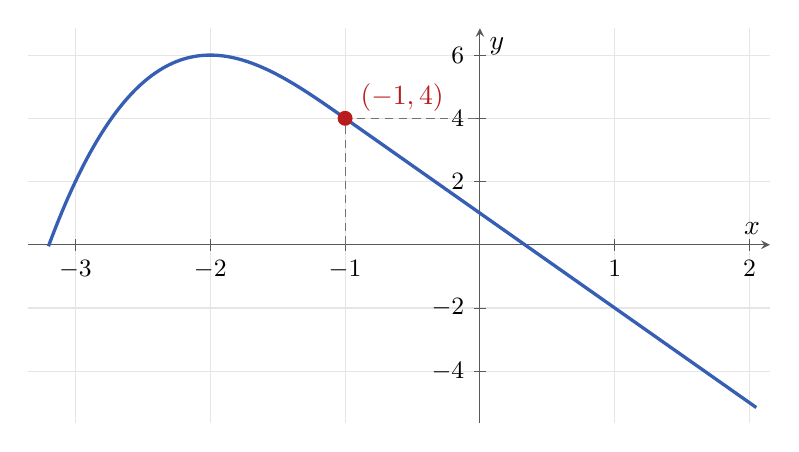
\begin{tikzpicture}
  \begin{axis}[
    width=11cm,
    height=6.6cm,
    axis lines=middle,
    xmin=-3.35,
    xmax=2.15,
    ymin=-5.65,
    ymax=6.85,
    xlabel={$x$},
    ylabel={$y$},
    xtick={-3,-2,-1,0,1,2},
    ytick={-4,-2,2,4,6},
    grid=major,
    grid style={black!10},
    axis line style={black!65},
    tick style={black!65},
    tick label style={font=\small},
    clip=false,
  ]
    \addplot[corba, very thick, domain=-3.2:-1, samples=150] {x^3+3*x^2+2};
    \addplot[corba, very thick, domain=-1:2.05, samples=80] {-3*x+1};
    \draw[guia, densely dashed]
      (axis cs:-1,0) -- (axis cs:-1,4) -- (axis cs:0,4);
    \addplot[only marks, mark=*, mark size=2.5pt, punt]
      coordinates {(-1,4)};
    \node[anchor=south west, text=punt, fill=white, inner sep=1.5pt]
      at (axis cs:-0.92,4.08) {$(-1,4)$};
  \end{axis}
\end{tikzpicture}
\end{document}
